\documentclass[]{article}

\usepackage{graphics}
\usepackage{geometry}
\usepackage{fontspec}
\usepackage{amsmath}
\usepackage{amssymb}
\usepackage{circuitikz}
\usepackage{minted2}

\setmainfont{NotoSans}
\geometry{margin=0.5in}
\graphicspath{{./images/}}
\DeclareGraphicsExtensions{.png}

\begin{document}

\author{Πλαστήρας Πέτρος}
\title{Εργαστήριο Λογικής Σχεδίασης - Εργασία 1 - Μέρος Β.2}
\date{25 Νοεμβρίου 2024}
\maketitle

Παρακάτω σας δίνεται ο κώδικας VHDL για την περιγραφή της οντότητας (entity) majority. Υλοποιήστε ένα κύ-
κλωμα το οποίο θα δέχεται τρεις εισόδους a, b, c και θα παράγει μια έξοδο y η οποία έχει την τιμή 1 όταν τουλάχιστον δυο από τις εισόδους έχουν την τιμή 1.
\inputminted{vhdl}{majority.vhdl}

\section{Πίνακας Αληθείας και εξισώσεις Boole}
Προκειμένου να υλοποιήσουμε το κύκλωμα με τις παραπάνω προδιαγραφές πρέπει πρώτα να
σχεδιάσουμε τον πίνακα αληθείας της συνάρτησης που περιγράφεται και στην συνέχεια
χρησιμοποιώντας τον να δημιουργήσουμε και να απλοποιήσουμε τις εξισώσεις Boole που προκύπτουν.
\begin{center}
	\begin{tabular}{ | c | c | c | c | c | }
		\hline \rule{0pt}{11pt} $A$ & $B$ & $C$ & $Y$ & $m_i$                         \\
		\hline \rule{0pt}{11pt} 0   & 0   & 0   & 0   & $\bar{A} * \bar{B} * \bar{C}$ \\
		\rule{0pt}{11pt} 0          & 0   & 1   & 0   & $\bar{A} * \bar{B} * C$       \\
		\rule{0pt}{11pt} 0          & 1   & 0   & 0   & $\bar{A} * B * \bar{C}$       \\
		\rule{0pt}{11pt} 0          & 1   & 1   & 1   & $\bar{A} * B * C$             \\
		\rule{0pt}{11pt} 1          & 0   & 0   & 0   & $A * \bar{B} * \bar{C}$       \\
		\rule{0pt}{11pt} 1          & 0   & 1   & 1   & $A * \bar{B} * C$             \\
		\rule{0pt}{11pt} 1          & 1   & 0   & 1   & $A * B * \bar{C}$             \\
		\rule{0pt}{11pt} 1          & 1   & 1   & 1   & $A * B * C$                   \\
		\hline
	\end{tabular}
\end{center}

Από το παραπάνω προκύπτει ως άθροισμα γινομένων η παρακάτω εξίσωση για το $Y$:
$$ Y = \bar{A} * B * C + A * \bar{B} * C + A * B * \bar{C} + A * B * C$$

Χρησιμοποιώντας τα θεωρήματα της άλγεβρας Boole, μπορούμε να απλοποιήσουμε το παραπάνω ως εξής:
\begin{align*}
	Y & = \bar{A} * B * C + A * \bar{B} * C + A * B * \bar{C} + A * B * C \\
	  & = \bar{A} * B * C + A * \bar{B} * C + A * B * (\bar{C} + C)       \\
	  & = \bar{A} * B * C + A * \bar{B} * C + A * B * 1                   \\
	  & = \bar{A} * B * C + A * \bar{B} * C + A * B                       \\
	  & = \bar{A} * B * C + A * \bar{B} * C + A * B + A * B               \\
	  & = (\bar{A} * B * C + A * B) + (A * \bar{B} * C + A * B)           \\
	  & = (\bar{A} * C + A) * B + A * (\bar{B} * C + B)                   \\
	  & = (C + A) * B + A * (C + B)                                       \\
	  & = B * C + A * B + A * C + A * B                                   \\
	  & = B * C + A * B + A * C                                           \\
\end{align*}

Στην παραπάνω υλοποίηση χρησιμοποιούνται 3 AND και 2 OR πύλες. Μπορούμε να μειώσουμε τον αριθμό των πυλών που χρησιμοποιούνται εφαρμόζοντας την επιμεριστική ιδιότητα σε δύο από τους 3 όρους:
\begin{align*}
	Y & = B * C + A * B + A * C \\
	  & = A * (B + C) + B * C   \\
\end{align*}

Τώρα χρησιμοποιούνται 2 πύλες AND και 2 πύλες OR.
\begin{minted}{vhdl}
-- filename: majority.vhd
\end{minted}
\inputminted{vhdl}{./assign_1/majority_old.vhdl}

\section{RTL Analysis}
Μπορούμε τώρα να κάνουμε RTL ανάλυση του παραπάνω κώδικα. Πατώντας 'Open Elaborated Design'
προκύπτει το παρακάτω διάγραμμα:

\begin{center}
	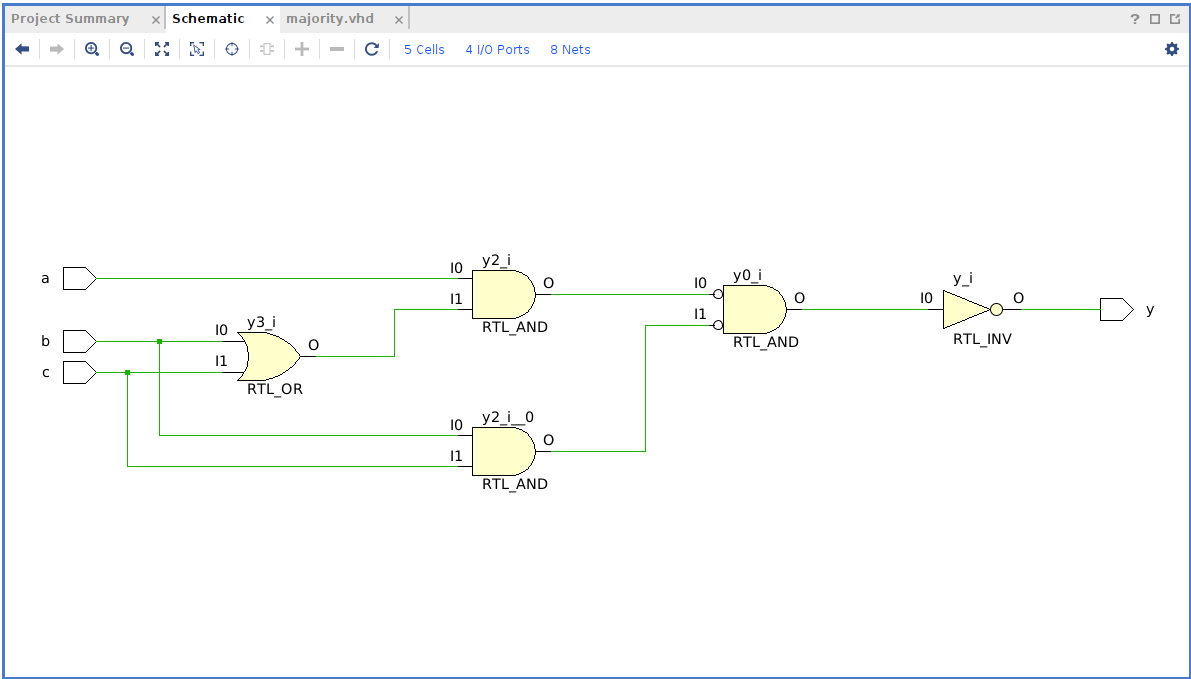
\includegraphics[width=10cm]{rtl_new.png}
\end{center}

Το κύκλωμα αποτελείται δύο πύλες OR δύο εισόδων και 2 πύλες AND δύο εισόδων όπως περιμέναμε.

\subsection{De Morgan side-quest}
Μπορούμε επίσης να μειώσουμε τον αριθμό από CMOS transistors που χρησιμοποιούνται, εφαρμόζοντας κανόνες De Morgan στην εξίσωση ώστε να αλλάξουμε όσες πύλες γίνεται σε NOR και NAND:
\begin{align*}
	Y & = A * (B + C) + B * C                                  \\
	  & = \overline{\overline{A * (B + C)} * \overline{B * C}} \\
\end{align*}

Η παραπάνω υλοποίηση αποτελείται από 3 πύλες NAND και μια πύλη OR.
Συνολικά έχει:
\begin{center}
	\begin{tabular}{| c | c |}
		\hline Πύλη   & Αριθμός CMOS Transistors \\
		\hline NAND-2 & 4                        \\
		NAND-2        & 4                        \\
		NAND-2        & 4                        \\
		OR-2          & 4 + 2 = 6                \\
		\hline Σύνολο & 4 + 4 + 4 + 6 = 18       \\
		\hline
	\end{tabular}
\end{center}

Το παρακάτω είναι ο κώδικας που αντιστοιχεί στην υλοποίηση του κυκλώματος χρησμιποιώντας τις εξισώσεις στις οποίες έχουν εφαρμοστεί κανόνες De Morgan:
\begin{minted}{vhdl}
-- file majority.vhd
\end{minted}
\inputminted{vhdl}{./assign_1/majority.vhdl}

Μετά από RTL ανάλυση του παραπάνω κώδικα προκύπτει το παρακάτω διάγραμμα:
\begin{center}
	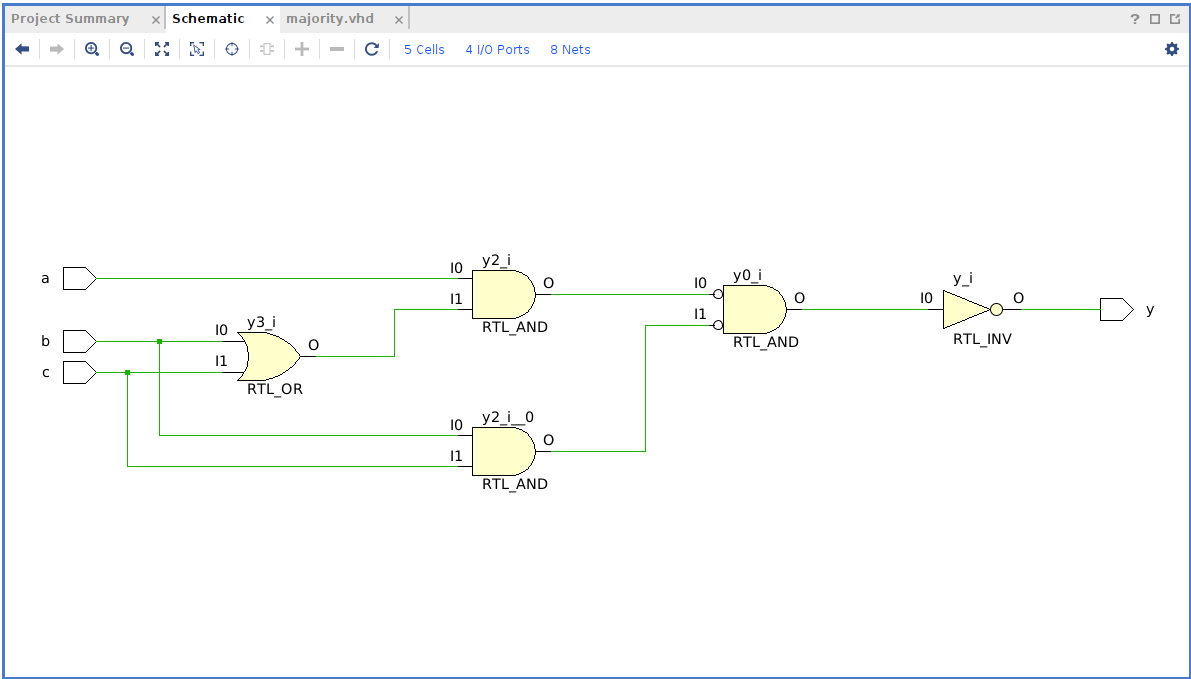
\includegraphics[width=10cm]{rtl_new.png}
\end{center}

Αφού χρησιμοποιήσαμε NAND στον κώδικα, περιμέναμε ότι θα χρησιμοποιούσε τις αντίστοιχες πύλες στο RTL διάγραμμα.
Ωστόσο αυτό δεν συνέβη και απλά χρησιμοποιήθηκαν αντιστροφείς. Αν προσπαθήσουμε να φτιάξουμε λοιπόν με την θεωρητικά
πιο αποδοτική μορφή του κώδικα το διάγραμμα, το Vivado απλά εισάγει 3 νέες πύλες. Το κύκλωμα αυτό χρησιμοποιεί 1 πύλη OR δύο εισόδων, 3 πύλες AND δύο εισόδων και 3 αντιστροφείς,
ενώ θα περιμέναμε να χρησιμοποιεί 1 πύλη OR δύο εισόδων και 3 NAND δύο εισόδων.

Για την τελική υλοποίηση θα χρησιμοποιηθεί η πρώτη μορφή μιας που έχει πιο απλό RTL διάγραμμα.
Φυσικά όποια μορφή και να χρησιμοποιήσουμε, αφού τελικά το κύκλωμα μετατρέπεται σε lookup tables κατά την σύνθεση δεν θα υπάρξει κάποια διαφορά(εφόσον ο αριθμός των LUT μένει ίδιος και στα δύο Schematics).

\section{Synthesis}
Πλέον μπορούμε να κάνουμε σύνθεση και κάνοντάς την προκύπτει το παρακάτω διάγραμμα:
\begin{center}
	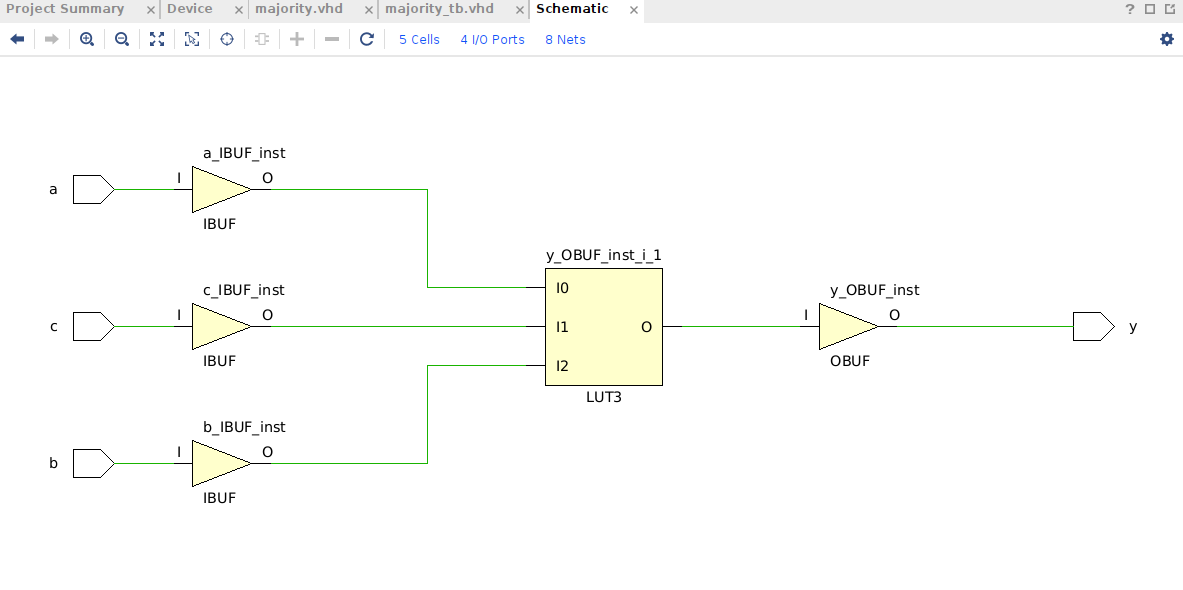
\includegraphics[width=10cm]{synthesis_schem.png}
\end{center}

Στο παραπάνω φαίνεται η τελική υλοποίηση της οντότητας μας με χρήση look-up table(LUT). Χρησιμοποιούμε μόνο
1 look-up table τριών εισόδων, στο οποίο έχει αποθηκευτεί ο πίνακας αληθείας της συνάρτησης. Χρησιμοποι-
ούνται επίσης 3 buffers για την ενίσχυση των σημάτων a, b και c πριν την είσοδό τους στο LUT καθώς κι ένα επιπλέον buffer για την ενίσχυση της εξόδου y.

\section{Simulation}
Για την προσομοίωση και τον έλεγχο της οντότητας majority υλοποιήθηκε και χρησιμοποιήθηκε η οντότητα majority\_tb με τον παρακάτω τρόπο:
\begin{minted}{vhdl}
-- file majority_tb.vhd
\end{minted}
\inputminted{vhdl}{./assign_1/majority_tb.vhdl}

Τρέχοντας το στάδιο του behavioral simulation προκύπτει η παρακάτω κυματομορφή:
\begin{center}
	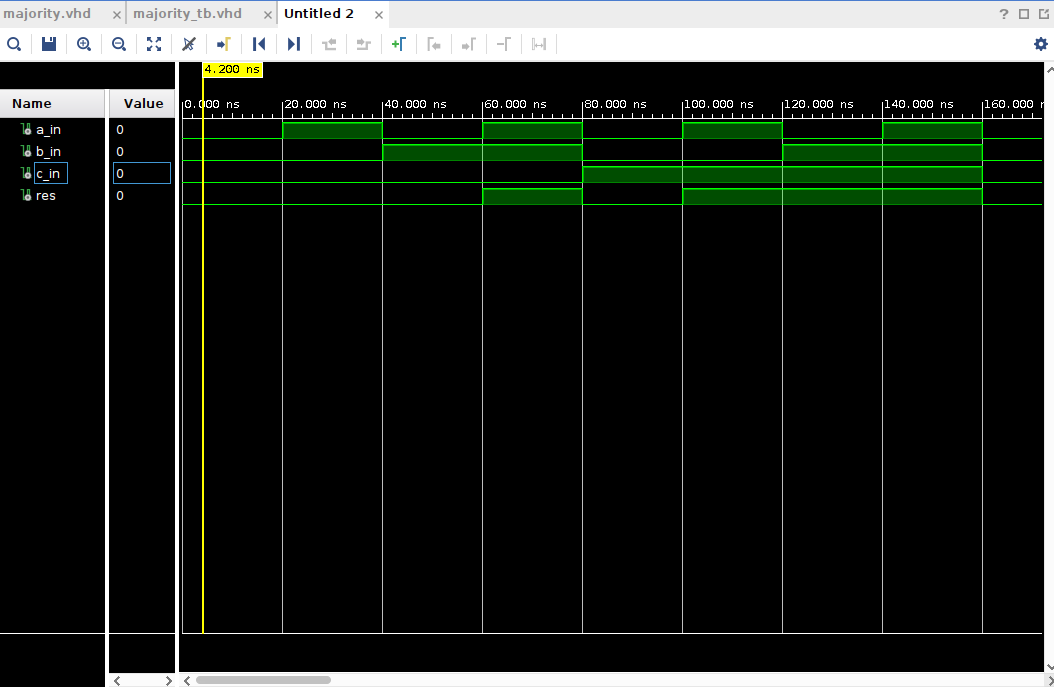
\includegraphics[width=10cm]{behavioral.png}
\end{center}

Μιας που ήδη έχουμε εκτελέσει το στάδιο της σύνθεσης και του behavioral simulation μας δίνεται πλέον η επιλογή να κάνουμε Post Synthesis Timing Simulation.
Τρέχοντας το προκύπτει η παρακάτω κυματομορφή:
\begin{center}
	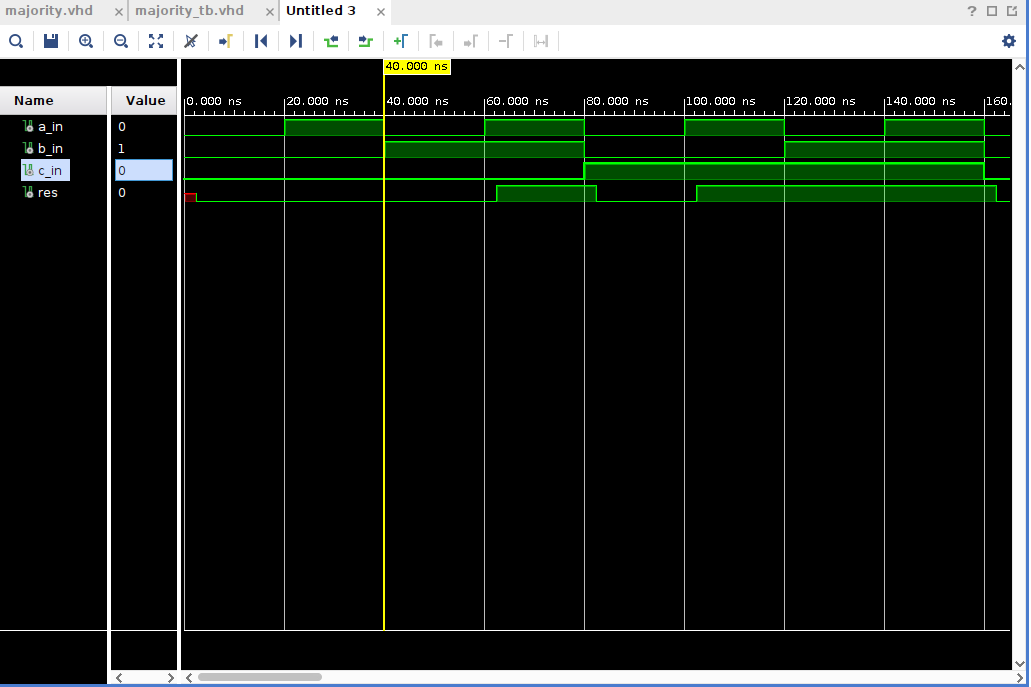
\includegraphics[width=10cm]{post_synthesis_timing.png}
\end{center}

Παρατηρούμε την διαφορά των δύο κυματομορφών. Ενώ στο behavioral simulation η μετάβαση από 0 σε 1 στο σήμα res γινόταν άμεσα εδώ
υπάρχει μια καθυστέρηση κατά την μεταβολή την τιμής του res, η οποία είναι της τάξης των $6ns$. Παρατηρούμε επίσης ότι κατά την αρχή
της εκτέλεσης υπάρχει ένα χρονικό διάστημα(επίσης της τάξης των $6ns$) κατά το οποίο το σήμα παίρνει την τιμή U η οποία υποδεικνύει ότι δεν έχει ανατεθεί τιμή στο σήμα.
Αυτό συμβαίνει επίσης λόγω της καθυστέρησης, η οποία, τελικά, σύμφωνα με τα παραπάνω φαίνεται να είναι περίπου $6ns$.
Όλα τα στοιχεία που χρησιμοποιούμε στο κύκλωμα προσθέτουν κάποια καθυστέρηση. Συνεπώς η καθυστέρηση των $6ns$ προκαλείται από το LUT, τα buffers και ακόμη και τα σύρματα που τα συνδέουν με τις εισόδους, τις εξόδους και μεταξύ τους.

\section{Correctness Check}
Τέλος, αρκεί να ελέγξουμε την λειτουργία του κυκλώματος, διασταυρώνοντας τον πίνακα αληθείας της συνάρτησης $Y$ με την κυματομορφή του behavioral simulation.
Παρατηρούμε ότι όταν 0 ή μία από τις εισόδους είναι 1, πράγμα που στην κυματομορφή συμβαίνει στα διαστήματα 0-20 ns, 20-40 ns, 40-60 ns και 80-100 ns το σήμα res που συνδέεται με το y της οντότητας είναι 0.
Συγκρίνοντας με τον πίνακα αληθείας, στις περιπτώσεις που οι είσοδοι είναι 000, 001, 010, 100 αντίστοιχα αναμένουμε το $Υ$ να είναι 0 και πράγματι αυτό ισχύει.

\textit{Σημείωση, ότι το a\_in της οντότητας προσομοίωσης, συνδέεται με το λιγότερο σημαντικό bit του αριθμού που χρησιμο- ποιούμε στο for-loop.
	Συνεπώς αντιστοιχεί στο $C$ στον πίνακα αληθείας. Αυτό ωστόσο δεν επηρεάζει το αποτέλεσμα μιας που το πρόβλημα είναι συμμετρικό ως προς τις εισόδους.}

Αν τώρα κοιτάξουμε τα υπόλοιπα διαστήματα δηλαδή 60-80 ns, 100-120 ns, 120-140 ns και 140-160 ns το σήμα res παίρνει την τιμή 1.
Οι περιπτώσεις αυτές αντιστοιχούν στις εισόδους 011, 101, 110, 111 οι οποίες στον πίνακα αληθείας πράγματι δίνουν στο $Y$ την τιμή 1.
Συνεπώς, το κύκλωμά μας λειτουργεί όπως θα περιμέναμε και τελικά η υλοποίηση της οντότητας majority είναι επιτυχής.

Ακολουθεί ένας πίνακας που συνοψίζει τα παραπάνω:
\begin{center}
	\begin{tabular}{|c|c|c|c|c|c|c|c|c|c}
		\hline Διάστημα  & a\_in & b\_in & c\_in & res & $A$ & $B$ & $C$ & $Y$ \\
		\hline $0-20 ns$ & 0     & 0     & 0     & 0   & 0   & 0   & 0   & 0   \\
		$20-40 ns$       & 1     & 0     & 0     & 0   & 0   & 0   & 1   & 0   \\
		$40-60 ns$       & 0     & 1     & 0     & 0   & 0   & 1   & 0   & 0   \\
		$60-80 ns$       & 1     & 1     & 0     & 1   & 0   & 1   & 1   & 1   \\
		$80-100 ns$      & 0     & 0     & 1     & 0   & 1   & 0   & 0   & 0   \\
		$100-120 ns$     & 1     & 0     & 1     & 1   & 1   & 0   & 1   & 1   \\
		$120-140 ns$     & 0     & 1     & 1     & 1   & 1   & 1   & 0   & 1   \\
		$140-160 ns$     & 1     & 1     & 1     & 1   & 1   & 1   & 1   & 1   \\
		\hline
	\end{tabular}
\end{center}

\end{document}
